\documentclass{article}
\usepackage{graphicx}
\graphicspath{{./figures/}}

\begin{document}

\title{Research in VGIS - Miniproject}
\author{Niclas Hjorth Stjernholm}

\maketitle

\section{Tensorflow Playground Tasks}
\subsection{Default settings}
\subsubsection*{Circles data}
The model converges very fast, within just around 150 iterations.
The data is divided in a simple pattern, and with the given two hidden layers with four and two neurons, the pattern created from the data is learned in a fast manner. With this low a complexity of pattern only a few neurons a used to learn the pattern and to classify the data.

\begin{figure}[h]
  \centering
  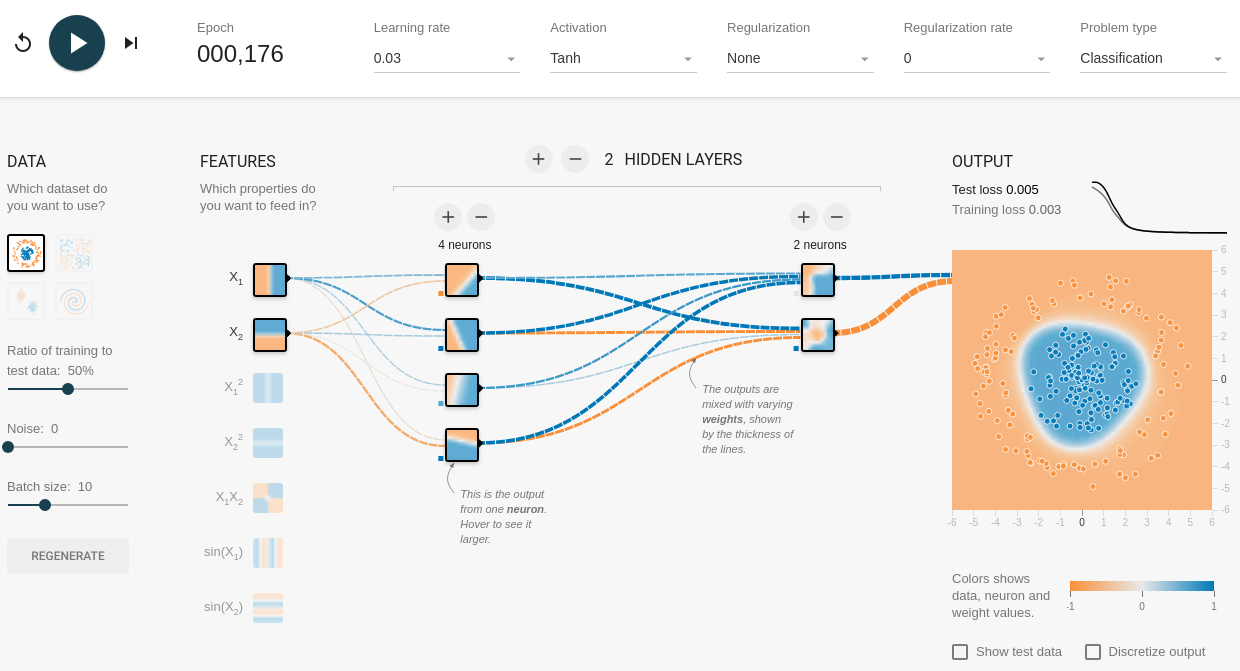
\includegraphics[width=0.8\textwidth]{default.png}
\end{figure}

\subsubsection*{Spiral data}
The model has a training loss of just around $0.3$ and a test loss even higher. This points to an underfitting which means the model is not able to properly fit to the data with the given capabilities.

\begin{figure}[h]
  \centering
  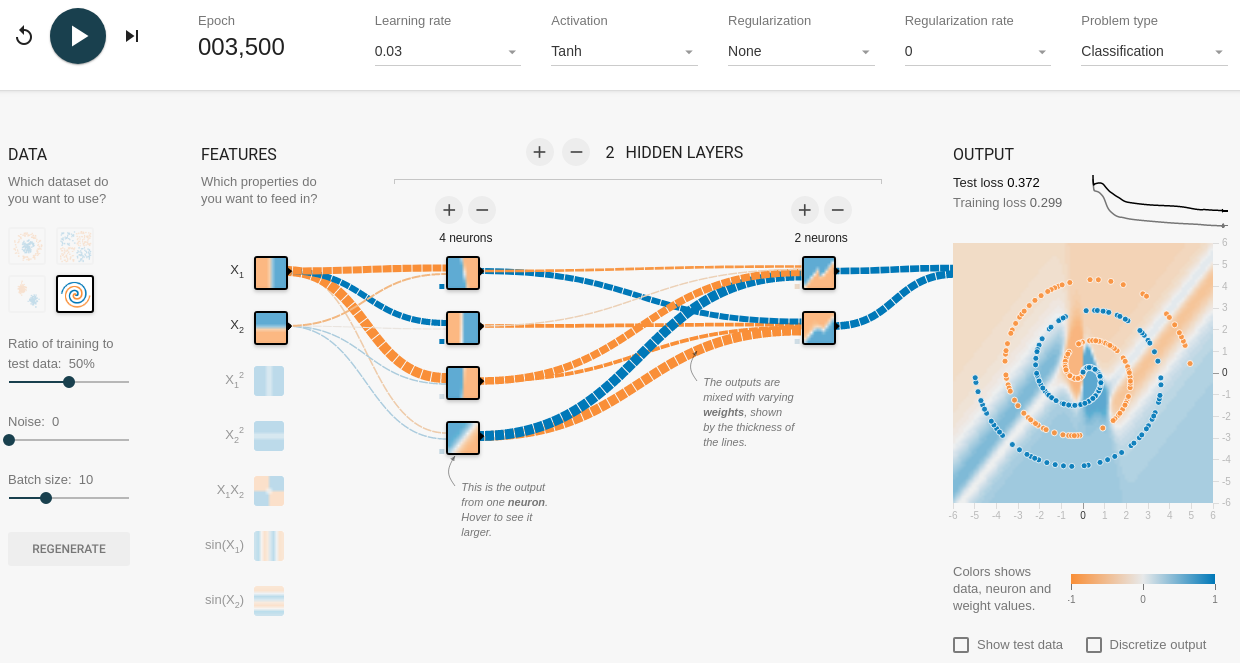
\includegraphics[width=0.8\textwidth]{default_spiral.png}
\end{figure}

\subsection{Alternated settings}
By increasing the amount of neurons to eight and adding another layer with six neurons, the model is able to converge to the data and attain a fitting shape.

\begin{figure}[h]
  \centering
  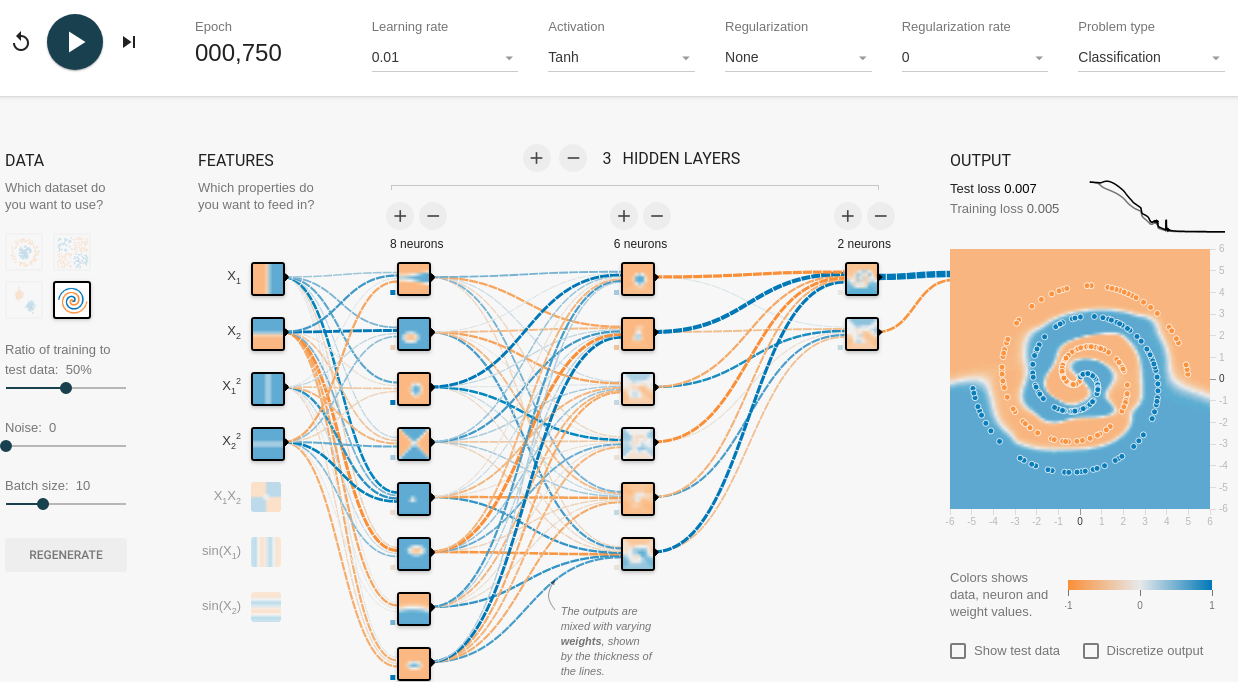
\includegraphics[width=0.8\textwidth]{alternated_spiral.png}
\end{figure}


\section{Quick, Draw! Doodle Recognition Challenge}

\end{document}
